\documentclass{article}
\usepackage[utf8]{inputenc}

\title{Chem132A: Lecture 04}
\author{Shane Flynn (swflynn@uci.edu) }
\date{10/6/17}


\usepackage{graphicx}
\usepackage{amsmath}
\usepackage{braket}
\usepackage[margin=0.7in]{geometry}
\usepackage{hyperref}


\newcommand{\be}{\begin{equation}}
\newcommand{\ee}{\end{equation}}
\newcommand{\benum}{\begin{enumerate}}
\newcommand{\eenum}{\end{enumerate}}
\newcommand{\pd}{\partial}

\begin{document}

\maketitle

\section*{Joule-Thompson Effect}
During the 19$^{th}$ Century Joule and Thomson became interested in measuring the temperature change associated with a gas expanding into a vacuum. 
From intuition you may expect a gas that expands to have an associated decrease in temperature (due to the work associated with the expansion). 
This intuition is useful, but not the entire story. 

If we consider the Enthalpy as a function of P and T; H(P,T) we can write a total differential of the Enthalpy as
\be
\begin{split}
dH &= \left(\frac{\pd H}{\pd P}\right)_T dP + \left(\frac{\pd H}{\pd T}\right)_P dT \\
dH &= \left(\frac{\pd H}{\pd P}\right)_T dP + C_P(T) dT
\end{split}
\ee

If we then consider an \textbf{Isenthalpic} Process (dH = 0), we can rearrange our equation to be. 
\be
\left(\frac{\pd H}{\pd P}\right)_T dP = -C_P(T) dT
\ee
If we then pretend that operators can be treated algebraically, we can divide by dP to find the following. 
\be
\begin{split}
\left(\frac{\pd H}{\pd P}\right)_T &= -C_P(T)\left(\frac{\pd T}{\pd P}\right)_H = -C_p(T) \mu\\
\mu &\equiv \left(\frac{\pd T}{\pd P}\right)_H 
\end{split}
\ee

For an ideal gas it can be shown that the Joule-Thomson coefficient is 0. 
If we find that $\mu >$ 0, it implies that the gas is cooling during the process, and $\mu <$ 0 would imply that the gas is heating up during the process. 

Because this process is defined as a gas expanding, the pressure must be decreasing. 
If the pressure is decreasing, and the temperature decreases, your derivative would be positive, implying your gas is cooling down as it expands. 
The same logic can be used for a negative Joule-Thomson coefficient; an increase in temperature upon expansion, and a decrease in pressure would imply the gas is heating up during the expansion, and the coefficient would be negative. 

If you are interested in understanding how a process can be made isenthalpic, please read the justification given on page 96 of the textbook. 

\subsection*{Interpreting the conditions}

\begin{figure}[h!]
\centering
\caption{Standard Joule-Thomson T,P Dependence: (Photo Atkins P.Chem)}
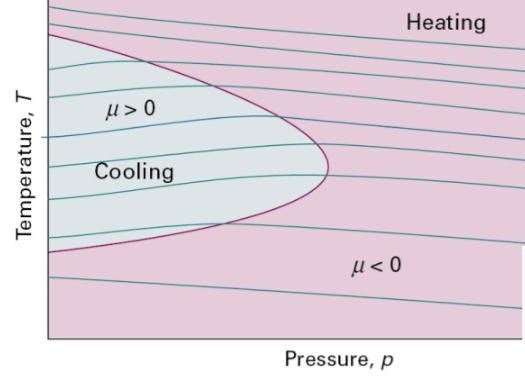
\includegraphics[width=0.5\textwidth]{JT.png}
\end{figure}

With this knowledge in hand you can investigate various temperatures and pressures to evaluate the Joule-Thomson coefficient (Figure 1).
Usually there are some conditions where you can generate cooling, and others where you can generate heating. 
The basis for this behavior are the underlying interactions that occur between molecules. 
In general, when atoms get too close to each-other they will start to repel.
You cannot have two atoms physically occupying the exact same space at the exact same time, and their charges will rapidly repel one-another as they get closer and closer. 

So when a system is placed under higher and higher pressures, the atoms will inevitably start to repel one-another. 
This means we can interpret a $\mu <$ 0 as a system where the dominate interactions between the atoms are repulsion's. 

Likewise a system with $\mu >$ 0 implies a system dominated by attractions. 
When the molecules are sufficiently far apart an overall attractive force will begin to pull them together (London-Dispersion forces). 
If the gas has a net attraction, and it needs to expand into a larger volume, some energy will be needed to move the atoms apart, causing the gas to decrease in temperature upon expansion. 

In day to day life we can usually stick something in the refrigerator to cool it. 
But if we want to cool a substance to extremely low temperatures (single digit Kelvin for example) we need to be a bit savvy in how to go about it efficiently. 
One method of doing this is to utilize the Joule-Thomson expansion effect. If you set the pressure and temperature within a device such that it cools your gas, you can make an efficient refrigerator. 

You make a closed device (Figure 2) with a compressor (increases pressure by reducing volume of the gas). 
Therefore the pressure at the top of the container is larger than the bottom. 
The gas then goes through a tube and exits the tube through a throttle (small volume output) into a lower pressure space.
This process is simply a Joule-Thomson expansion of the gas we are trying to cool. 
If the conditions are such that the gas cools($\mu>$0), this process can simply be repeated, with each iteration of the process the gas will be cooled more and more until eventually liquefying. 

The gas within at the top of the tube, before the throttle, has not undergone the expansion yet so, it will be at a higher temperature and pressure. 
The tube is not isolated, as the gas cools, the environment cools causing the temperature of the tube to decrease further, which then decreases the temperature of the gas more. 
Nothing can be done for free, the heat exchanger is used to manage excess heat for this process. 

\begin{figure}[h!]
\centering
\caption{Linde Refrigerator Application: (Photo Atkins P.Chem)}
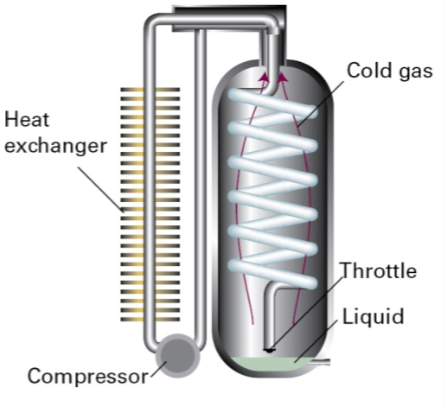
\includegraphics[width=0.5\textwidth]{Linde_ref.png}
\end{figure}


















\end{document}